\section{Liberating the Guardian Angel}

\begin{quotationx}
Between the angelic nature, which is an intellectual thing, and the human soul there is no step, but they are both
almost continuous in the order of gradation. … Thus we are to suppose and firmly to believe, that a man may be so noble,
and of such lofty condition, that he shall be almost an angel. \flright{\textsc{Dante}, \emph{Convivio}, VII, 3}

Nearly all that has been said theologically of the angels can be said metaphysically of the superior states of the
being, just as in the astrological symbolism of the Middle Ages the ‘heavens’, that is to say
the various planetary and stellar spheres, represent these same states and also the initiatic degrees to which their
realization corresponds \flright{\textsc{Rene Guenon}, \emph{Multiple States of Being}}

In flowing and running water, in mists dissolving into water, also in the winds and the lightning flashing through the
air, in all these, you have to look for the physical body of Angelic beings. The difficulty for man consists in his
fixed idea that a physical body must necessarily have a definite outline. It is difficult for a man to say to himself:
I see fog rising, I see a stream of water dissolving into spray, I stand in the blowing wind, I see lightning dart from
the clouds, and I know that all these are revelations of Angels; behind this physical body, which is by no means so
limited as the human one I have to recognise the spirit. \flright{\textsc{Rudolf Steiner}, \emph{The Spiritual Hierarchies}}
\end{quotationx}

As long as the human being is regarded as just one species in the Animal Kingdom, there will be no possibility of
understanding. Humanity is a Kingdom in itself; hence, humans require a cladistics distinct from merely biological
categories. Starting with some early notes, and developed over time, Valentin Tomberg observed a clade based on the
depth of a person's awareness of Self and his relationship to angelic hierarchies. There are three such
classifications of the human being.

\begin{itemize}
\item \textsc{Love class}: Those in this class have realized a permanent sense of I and are victorious. They live only
for humanity and have come to help. These are in direct contact with the 1st hierarchy. 
\item \textsc{Conscience class}: People in this class consciously take part in the conflict between good and evil. They
have developed a sense of the I and are led by the 2nd hierarchy. 
\item \textsc{Karmic class}: These have not developed a real sense of I and are victims of the curses resulting from the
Fall. The people of the third class are all still experiencing their own karma and looking for their real purpose in
life. These are under the leadership of the 3rd hierarchy. 
\end{itemize}

Finally there are those who are unable to develop a sense of I at this time.

\paragraph{Spiritual Baptism}

\begin{wrapfigure}{tr}{.3\textwidth}
 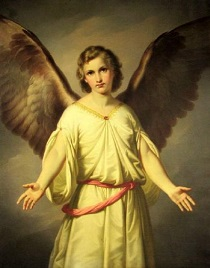
\includegraphics[scale=.6]{a20220407LiberatingtheGuardianAngel-img001.jpg} 
\caption{Archangel Gabriel}
\end{wrapfigure}

Tomberg describes a “spiritual baptism” which takes place before birth and prepares the soul for its life mission. The
experience differs for each class.

For people of the 3rd \textbf{Karmic Class}, spiritual baptism consists in being consciously reminded of the fate that
they will experience as karma.

For people of the 2nd \textbf{Conscience Class}, spiritual baptism brings to awareness a request from the spiritual
world to focus attention on a task, or to develop knowledge of something in the spiritual world.

For people of the 1st \textbf{Love Class}, baptism consists in the soul telling the hierarchy what it is ready to
accomplish.

\paragraph{Angelic Bodies}
In order to understand higher states available to humans, it is first necessary to be clear about how the angelic states
are related to the human. The lowest order, the Angels proper, share the ether body, astral body, an intellectual soul
(the “I”) with man. Hence Angels cannot understand man's physical nature, yet are familiar with the
corresponding states of the soul.

Archangels, then, like the angels have no physical body, but neither do they have an etheric body. Hence, they relate to
the human on the astral level and above.

Of course, the various angels possess all the higher states of man, who, on the other hand, must work in order to reach
those higher states.

\paragraph{Karmic Class}
In the \emph{Meditations on the Tarot}, Tomberg describes the process of ascending from the third class to the first.
When the soul is ready to move upward, the guardian Angel withdraws.

\begin{quotex}
This is called in Christian Hermeticism “liberating the guardian Angel”. The guardian Angel is freed — often
in order to be able to acquire new missions — when the soul has acquired the disposition of its part of
“likeness” in order to experience the Divine more intimately and more immediately, which corresponds to another
hierarchical degree. Then it is an Archangel who replaces the freed guardian Angel. Human beings whose guardian is an
Archangel have not only new experiences of the Divine in their inner life, but also receive a new and objective
vocation. They become representatives of a human group — a nation or a human karmic community — which means that from this time onwards their actions will no longer be purely personal but will at the same time have
significance and value for those of the human community that they represent. 

\end{quotex}
\paragraph{Conscience Class}
Those of the second class are under the guidance of the second hierarchy. Tomberg elucidates:

\begin{quotex}
It also happens sometimes that the Archangel is freed as well. Then an entity from the hierarchy of Powers (Exusiai)
replaces the Archangel. The human being then becomes a representative of the future of humanity. He lives in the
present what mankind someday is due to experience in future centuries. 

\end{quotex}
Unlike those in the Karmic class, who are passive to the forces of life, these people have a sense of I and consciously
engage in spiritual warfare. They war against the spirits of the air from below while the Exusiai battle them from
above.

The future of mankind depends on this outcome.

\paragraph{Love Class}
Those in the first class have a higher mission, and are under the guidance of the highest angelic levels. He uses Saint
Francis of Assisi as an example.

\begin{quotex}
Lastly, a guardian Elohim — and there are many of them — can also be freed. Then it is an entity
of the first hierarchy, a Seraphim, who replaces him. It was so for \textbf{Saint Francis of Assisi}. The Seraphim who
gave him the teaching of the Crucifixion whereby he gained the stigmata — the Seraphim in the vision of St.
Francis — was his guardian. This is why Saint Francis represents more than mankind; what he represents is
“divinised humanity”. 

\end{quotex}

\hfill

Sources:\newline
\emph{Chakra Werk} by \textbf{Willi Seiß}.\newline
\emph{Meditations on the Old Testament} by \textbf{Valentin Tomberg}\newline
\emph{Meditations on the Tarot} by \textbf{Valentin Tomberg}


\flright{\itshape Posted on 2022-04-27 by Cologero}

\begin{center}* * *\end{center}


\begin{footnotesize}\begin{sffamily}

\texttt{Janet Martha on 2022-04-30 at 12:44 said: }

“The personal God is the angel. The angel is the space in which the Godhead shows itself in your heart.” David
Nieuwejaers, rephrasing Henri Corbin.


\end{sffamily}\end{footnotesize}